\documentclass{article}
\usepackage[utf8]{inputenc}
\usepackage{graphicx}
\usepackage{amsmath}
\usepackage{amssymb}
\usepackage{hyperref}
\usepackage{enumerate}

\usepackage[backend=bibtex]{biblatex}
\addbibresource{referencias.bib}

\title{Predicción del comportamiento de una enfermedad simulada en autómatas celulares con un algoritmo propuesto en redes neuronales}
% Titulo v1: Diseño e implementación de un algoritmo en redes neuronales que permita realizar predicciones sobre el comportamiento de una enfermedad simulada en autómatas celulares.
% Titulo v2:  Predicción del comportamiento de una enfermedad simulada en autómatas celulares con un algoritmo propuesto en redes neuronales

%\author{}
\date{\today}

\begin{document}

\maketitle
% \section{Introducción}
% \newpage
\section{Formulación del problema}

Las matemáticas han sido pieza fundamental en el estudio epidemiológico. El cual busca predecir el comportamiento de una enfermedad para mitigar su impacto, tomando medidas de control y prevención. 

Se considera como punto de partida el modelo descrito por Kermack y McKendrick en 1927, también conocido como modelo SIR, en el que se establecen relaciones entre tres estados de una enfermedad (Susceptible-Infectado-Recuperado) y se implementan los conceptos de tasa de contagio y de recuperación \cite{malariaSIR}. Desde entonces se han desarrollado múltiples variaciones sobre el modelo SIR, con el objetivo de analizar diferentes tipos de enfermedades de una manera más precisa, considerando por ejemplo diferentes estados, tasas de natalidad y mortalidad, entre otros \cite{diego2010}.

Por otra parte y debido a los avances tecnológicos de las últimas décadas, se han desarrollado modelos y simulaciones que permiten analizar características que no eran posibles con los modelos anteriormente mencionados. Por ejemplo, patrones de movilidad \cite{colaGNN, epidemiologicalNeuralNetwork}, disminución en la cantidad de contagios debido a un aislamiento preventivo \cite{stayHome}, contagios de individuo a individuo \cite{heterogeneousPopulation} e interacciones en masa \cite{combiningGraph, transfer2021}, la mayoría realizadas con una fuerte influencia de las redes neuronales y complejas, apoyadas fuertemente sobre la teoría de grafos. 

La inexistencia de un algoritmo predictivo que tenga en cuenta las interacciones más cercadas de cada individuo, es un problema que se ha evidenciado principalmente, a causa de la naturaleza de las bases de datos disponibles.

% \newpage
\section{Justificación}

A pesar del fuerte acercamiento de los modelos epidemiológicos a las dinámicas sociales con la llegada del coronavirus, se consideran interacciones a escalas que podrían ser mayores a las que se contagia la enfermedad, si bien existen modelos que analizan dinámicas de persona a persona, sus capacidades predictivas resultan limitadas por la naturaleza con la que se generan las bases de datos, como ocurre en \cite{combiningGraph,transfer2021}.

Teniendo en cuenta la aplicabilidad de los autómatas celulares y las cualidades predictivas de los modelos en redes neuronales, se pretende simular el comportamiento de una enfermedad y desarrollar un algoritmo que permita realizar pronósticos sobre su comportamiento, para responder a la pregunta: ¿Qué impacto tienen las relaciones sociales cercanas, en la propagación de una enfermedad?

Este trabajo permitirá comprender de manera más certera, como las interacciones de las personas afectan la propagación de alguna enfermedad y podrá establecer características para construir las bases de datos, que pueden dar lugar a análisis predictivos más realistas. Así mismo, se abre la puerta a que se propongan diferentes algoritmos con el fin de obtener diferentes resultados óptimos que alimenten el estudio epidemiológico.


% \newpage
\section{Objetivos}
\section*{Objetivo general}
Diseñar un algoritmo en redes neuronales que permita realizar pronósticos en el comportamiento de una enfermedad simulada con autómatas celulares, teniendo en cuenta aspectos topológicos que describan las interacciones entre individuos.
\section*{Objetivos específicos}
\begin{itemize}
    \item Establecer la topología que describa las relaciones entre autómatas.
    \item Diseñar el conjunto de reglas probabilísticas que modelen las dinámicas de la enfermedad.
    \item Implementar las dinámicas de comportamiento de los agentes en Python, con el propósito de simular la propagación de la enfermedad. 
    \item Identificar el conjunto de datos de entrenamiento adecuado para el algoritmo en redes neuronales.
    \item Definir las métricas que se van a monitorear con el algoritmo en redes neuronales.
    \item Diseñar e implementar un algoritmo en redes neuronales que permita realizar pronósticos para el comportamiento de la enfermedad simulada.
    \item Validar el comportamiento del algoritmo en ambientes topológicos distintos.
\end{itemize}

% \newpage
\section{Antecedentes}
Los modelos epidemiológicos compartiméntales clásicos, descritos por Kermack y McKendrick, han sido fuente de numerosos estudios y simulaciones relacionadas con el estudio epidemiológico. Como caso particular, encontramos el modelo propuesto por Fuentes y Kuperman en \cite{spatialDependences}, el cual permite estudiar la evolución de un núcleo de infectividad en varias condiciones y para dos tipos de enfermedades epidemiológicamente distintas, en autómatas celulares. A diferencia de los modelos clásicos en ecuaciones diferenciales \cite{diego2010}, proponen un conjunto de reglas de evolución para determinar el estado de un individuo en función de su propio estado y el de sus vecinos en pasos de tiempo anteriores, considerando un radio de "interacción".

En trabajos como el de Mikler-Venkatachalam-Abbas en \cite{globalStochastic}, los autómatas son interpretados como regiones, de modo que se puedan tener en cuenta factores geográficos, demográficos, de medio ambiente y patrones de migración, usando un autómata celular estocástico global (GSCA). Algo comparable se ve en \cite{modelingEpidemicsUsingCA}, en donde H. White, Martín del Rey y G. Rodríguez implementan la misma noción de autómata espacial, para analizar entre otras cosas el proceso de vacunación para una enfermedad modelada con un enfoque determinista.

Un enfoque diferente se ve en \cite{entropyDynamics}, en donde Marr y Hutt se enfatizan en la relación entre topología y teoría de grafos, para analizar dinámicas de redes biológicas. Mostrando que la distribución de grados puede estar relacionada con las propiedades dinámicas de la red, además de mencionar posibles mejoras basadas en ideas de topología de redes para analizar diferentes grados de entropía.

Encontramos también aplicaciones entre la teoría de redes y la epidemiología. Moo Kim realiza un análisis interesante para la propagación de enfermedades en redes complejas, puntualmente en la red de Barabasi-Albert, presente en diversas redes reales \cite{redesComplejas}. Realiza además, una implementación de los modelos compartimentales clásicos en redes regulares y complejas.

Desplazándonos un poco a la teoría de redes neuronales y los procesos de machine-learning, encontramos trabajos como el de Schmidt en \cite{schmidt2019}, en donde implementa una red neuronal artificial, basada en modelos compartimentales para predecir la propagación del virus de la influenza, para posteriormente realizar una comparación con un modelo de regresión lineal múltiple. 

Otra aplicación interesante es el modelo desarrollado en \cite{colaGNN}, el cual se centra en la predicción de los ILI a largo plazo, usando datos con un rango de tiempo limitado a 20 semanas. Teniendo presente la perdida de información temporal, exploran un modelo de propagación en grafos con representaciones espaciales. Usan además, las redes neuronales recurrentes para capturar las dependencias secuenciales en los datos de las series temporales locales y diseñan un modulo de convolución temporal para extraer automáticamente las dependencias temporales cortas y largas de los datos de series temporales de múltiples localizaciones.

La reciente aparición del coronavirus a finales del 2019, ha incentivado estudios que proponen diversos enfoques basados en redes neuronales convolucionales de grafos (GCNs), memorias de corto plazo (LSTMs) y modelos de aprendizaje de transferencia basados en el meta-aprendizaje (MAML) \cite{combiningGraph, epidemiologicalNeuralNetwork}. Mientras que en \cite{epidemiologicalNeuralNetwork} proponen un modelo basado en machine-learning para estimar los parámetros de un modelo epidemiológico que se ajusta a tendencias observadas sobre el movimiento de individuos, en \cite{combiningGraph} proponen un enfoque de fusión entre redes neuronales basadas en grafos y modelos epidemiológicos para combinar directamente los datos de movilidad diádica y conectividad derivadas de Facebook con información estructural y espacial de distritos alemanes.

Panagopoulos, Nikolentzos y Michalis Vazirgiannis realizan un trabajo comparable en \cite{transfer2021}, en donde se centran en predecir el comportamiento de la enfermedad basándose en los datos de movilidad de masa, y consideran la movilidad dentro de una región como un indicador de interacción. Exponen además, la inexistencia de una base de datos que considere las posibles interacciones entre individuos y sus implicaciones.

Después de revisar diferentes desarrollos en el campo de la epidemiología, se ratifica la importancia de un análisis predictivo que tenga en cuenta las relaciones o interacciones más cercanas, de modo que se establezcan estrategias de prevención y contención mucho más certeras.

\newpage
\section{Metodología}
Este proyecto estará dividido en cuatro fases principales, que se articulan entre sí y con los objetivos específicos del proyecto. Las fases se ejecutarán en forma secuencial y cada una de ellas generará una serie de módulos concretos que servirán de insumo a las fases subsecuentes. A continuación, se describe brevemente cada una de las fases metodológicas junto con la articulación con los objetivos específicos del proyecto:

\begin{figure}[h.]
  \centering
    \includegraphics[width=0.95\textwidth]{Imagenes/metodologia.PNG}
\end{figure}

\subsubsection*{Fase 1: Definición de reglas de interacción entre individuos.}
La primera fase del proyecto consistirá en definir las interacciones para los diferentes participantes dentro de nuestra investigación. Partiremos de la definición de una topología definida por un sistema de vecindades locales, con el fin de simular las relaciones sociales entre individuos.

Posteriormente se hará uso de reglas totalísticas para definir las dinámicas de la enfermedad, teniendo en cuenta los comportamientos locales para cada individuo. 
\subsubsection*{Fase 2: Simulación de la enfermedad.}
Una vez se establezcan las dinámicas de la enfermedad y de los individuos, se implementarán en Python usando las librerías: numpy, random, matplotlib, entre otras, para cálculos con arreglos numéricos, valores aleatorios y gráficos respectivamente.
\subsubsection*{Fase 3: Diseño e implementación del algoritmo en redes neuronales.}
Durante esta fase se definirán las métricas de interés para el estudio epidemiológico y se establecerán las neuronas que harán parte del algoritmo. 

Al igual que la simulación de la enfermedad, el algoritmo definido en esta etapa, se desarrollará sobre Python usando las diferentes librerías disponibles para redes neuronales. 
\subsubsection*{Fase 4: Entrenamiento del algoritmo y desarrollo de pruebas.}
Para entrenar el algoritmo propuesto, se tomarán las bases de datos simulados en la fase 2. Posteriormente se realizarán modificaciones en los parámetros de la enfermedad, el sistema de vecindades locales y la condición de frontera del conjunto de individuos, para poner a prueba las cualidades predictivas del algoritmo propuesto.  
% \newpage 
\section{Cronograma}
\begin{figure}[h.]
  \centering
    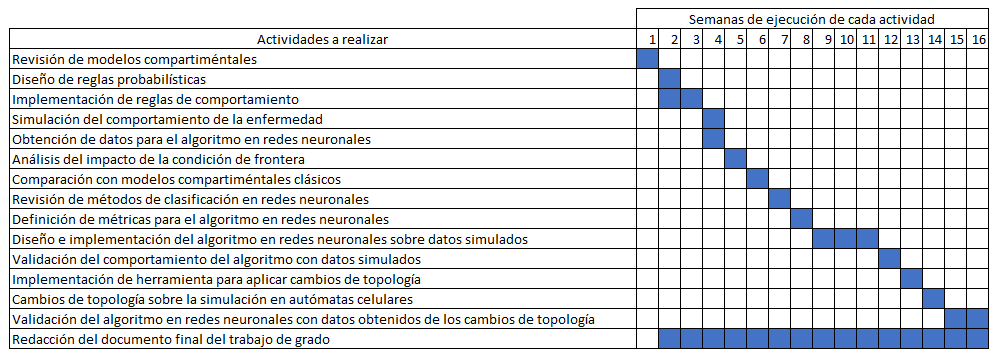
\includegraphics[width=1.1\textwidth]{Imagenes/cronograma.PNG}
\end{figure}
% \newpage
\printbibliography
\end{document}
